%========================================
% LESSON CONTENT: Ecuaciones Lineales en Dos Variables
%========================================

\lesson{Ecuaciones Lineales en Dos Variables}

%========================================
% SECTION 11.1: Introducción
%========================================
\subsectiontitle{Introducción a las Ecuaciones Lineales en Dos Variables}

\begin{definition}
\textbf{Ecuación Lineal en Dos Variables:}

Una ecuación lineal en dos variables es una ecuación que se puede escribir en la forma:

$$\boxed{Ax + By = C}$$

donde:
\begin{itemize}
    \item $A$, $B$ y $C$ son constantes (números reales)
    \item $A$ y $B$ no son ambos cero
    \item $x$ e $y$ son las variables
\end{itemize}

Esta forma se conoce como \textbf{forma estándar} de una ecuación lineal.
\end{definition}

\textbf{Ejemplos de ecuaciones lineales en dos variables:}
\begin{itemize}
    \item $2x + 3y = 6$ \quad (donde $A = 2$, $B = 3$, $C = 6$)
    \item $x - 4y = 8$ \quad (donde $A = 1$, $B = -4$, $C = 8$)
    \item $5x = 10$ \quad (donde $A = 5$, $B = 0$, $C = 10$)
    \item $-3y = 9$ \quad (donde $A = 0$, $B = -3$, $C = 9$)
\end{itemize}

\textbf{Observación importante:} A diferencia de las ecuaciones lineales con una variable (que tienen una solución), las ecuaciones lineales con dos variables tienen un \textbf{número infinito de soluciones}.

\newpage
%========================================
% SECTION 11.2: Soluciones y Gráficas
%========================================
\subsectiontitle{Soluciones y Gráficas de Ecuaciones Lineales}

\begin{definition}
\textbf{Solución de una Ecuación Lineal en Dos Variables:}

Una solución de una ecuación lineal en dos variables es un \textbf{par ordenado} $(x, y)$ que satisface la ecuación cuando los valores se sustituyen en ella.

Estas soluciones se pueden representar como \textbf{puntos} en el sistema de coordenadas rectangulares (visto en la Lección 10).
\end{definition}

\subsubsection*{Método de Tabulación}

Para encontrar soluciones de una ecuación lineal:
\begin{enumerate}
    \item Elija un valor para una de las variables (usualmente $x$)
    \item Sustituya ese valor en la ecuación
    \item Resuelva para la otra variable ($y$)
    \item El par ordenado $(x, y)$ es una solución
    \item Repita el proceso para obtener más soluciones
\end{enumerate}

\begin{example}
\textbf{Encontrar soluciones de una ecuación lineal}

Dada la ecuación $2x + 3y = 6$, encuentre al menos tres soluciones.

\textbf{Solución:}

\textbf{Para $x = 0$:}
\begin{align*}
2(0) + 3y &= 6 \\
3y &= 6 \\
y &= 2
\end{align*}
Solución: $(0, 2)$

\textbf{Para $x = 3$:}
\begin{align*}
2(3) + 3y &= 6 \\
6 + 3y &= 6 \\
3y &= 0 \\
y &= 0
\end{align*}
Solución: $(3, 0)$

\textbf{Para $x = -3$:}
\begin{align*}
2(-3) + 3y &= 6 \\
-6 + 3y &= 6 \\
3y &= 12 \\
y &= 4
\end{align*}
Solución: $(-3, 4)$

\textbf{Tabla de valores:}

\begin{center}
\begin{tabular}{|c|c|c|}
\hline
$x$ & $y$ & Punto $(x, y)$ \\
\hline
$-3$ & $4$ & $(-3, 4)$ \\
\hline
$0$ & $2$ & $(0, 2)$ \\
\hline
$3$ & $0$ & $(3, 0)$ \\
\hline
$6$ & $-2$ & $(6, -2)$ \\
\hline
$9$ & $-4$ & $(9, -4)$ \\
\hline
\end{tabular}
\end{center}
\end{example}

\newpage

\subsubsection*{Gráfica de una Ecuación Lineal}

\begin{theorem}
\textbf{Propiedad Fundamental:}

La gráfica de cualquier ecuación lineal en dos variables es una \textbf{línea recta}.

Para graficar una ecuación lineal:
\begin{enumerate}
    \item Encuentre al menos dos puntos (soluciones) de la ecuación
    \item Grafique estos puntos en el plano de coordenadas
    \item Trace una línea recta que pase por todos los puntos
\end{enumerate}

\textbf{Nota:} Aunque solo se necesitan dos puntos para definir una recta, es recomendable encontrar un tercer punto como verificación.
\end{theorem}

% Graphical representation of 2x + 3y = 6
\begin{center}
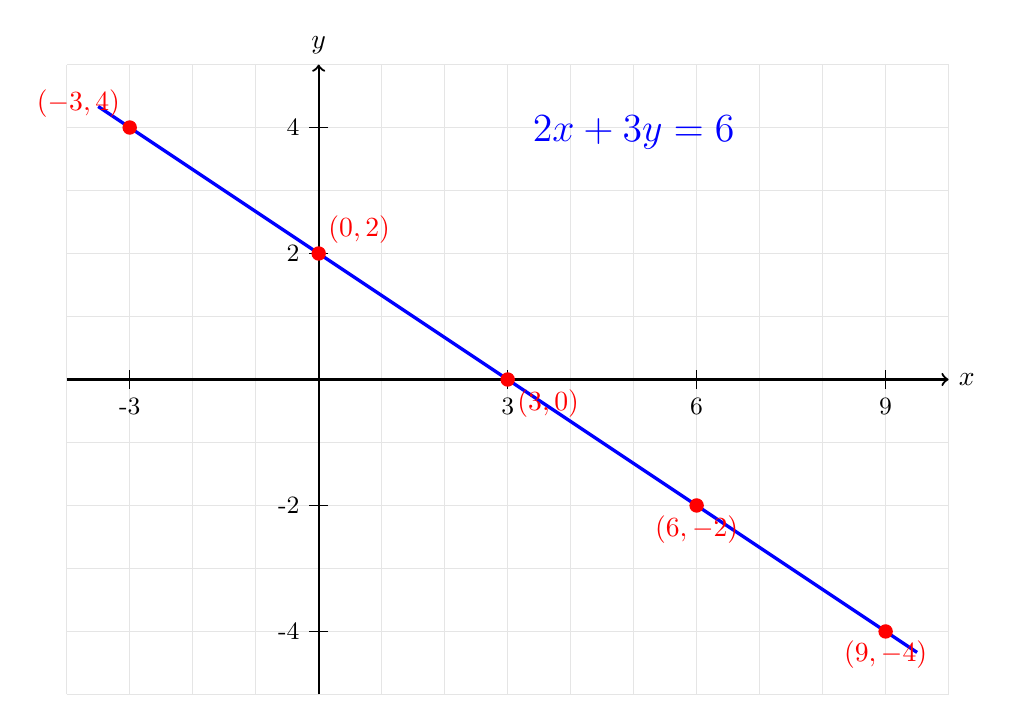
\begin{tikzpicture}[scale=0.8]
    % Grid
    \draw[gray!20, very thin] (-4,-5) grid (10,5);

    % Axes
    \draw[->, thick] (-4,0) -- (10,0) node[right] {$x$};
    \draw[->, thick] (0,-5) -- (0,5) node[above] {$y$};

    % Axis labels
    \foreach \x in {-3,3,6,9}
        \draw (\x,0.15) -- (\x,-0.15) node[below, font=\small] {\x};
    \foreach \y in {-4,-2,2,4}
        \draw (0.15,\y) -- (-0.15,\y) node[left, font=\small] {\y};

    % Plot the line 2x + 3y = 6
    \draw[blue, very thick, domain=-3.5:9.5] plot (\x, {(6-2*\x)/3});

    % Plot the points from table
    \filldraw[red] (-3,4) circle (3pt);
    \node[red, above left] at (-3,4) {$(-3,4)$};

    \filldraw[red] (0,2) circle (3pt);
    \node[red, above right] at (0,2) {$(0,2)$};

    \filldraw[red] (3,0) circle (3pt);
    \node[red, below right] at (3,0) {$(3,0)$};

    \filldraw[red] (6,-2) circle (3pt);
    \node[red, below] at (6,-2) {$(6,-2)$};

    \filldraw[red] (9,-4) circle (3pt);
    \node[red, below] at (9,-4) {$(9,-4)$};

    % Equation label
    \node[blue, above] at (5,3.5) {\Large $2x + 3y = 6$};
\end{tikzpicture}
\end{center}

\newpage
%========================================
% SECTION 11.3: Intersecciones con los Ejes
%========================================
\subsectiontitle{Intersecciones con los Ejes}

Las intersecciones con los ejes son puntos especiales que facilitan la gráfica de ecuaciones lineales.

\begin{definition}
\textbf{Intersecciones (Interceptos):}

\begin{itemize}
    \item \textbf{Intersección con el eje $x$ (x-intercept):} Las coordenadas $x$ de los puntos donde la gráfica interseca al eje $x$.
    \begin{itemize}
        \item Para encontrarla: Haga $y = 0$ y despeje $x$
        \item El punto tiene la forma $(a, 0)$
    \end{itemize}

    \item \textbf{Intersección con el eje $y$ (y-intercept):} Las coordenadas $y$ de los puntos donde la gráfica interseca al eje $y$.
    \begin{itemize}
        \item Para encontrarla: Haga $x = 0$ y despeje $y$
        \item El punto tiene la forma $(0, b)$
    \end{itemize}
\end{itemize}
\end{definition}

% Visual representation of intercepts
\begin{center}
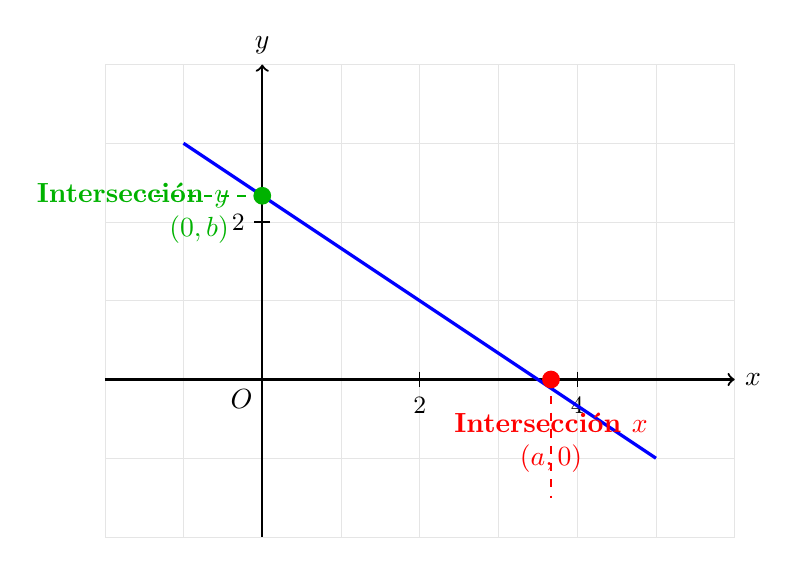
\begin{tikzpicture}[scale=1.0]
    % Grid
    \draw[gray!20, very thin] (-2,-2) grid (6,4);

    % Axes
    \draw[->, thick] (-2,0) -- (6,0) node[right] {$x$};
    \draw[->, thick] (0,-2) -- (0,4) node[above] {$y$};

    % Axis labels
    \foreach \x in {2,4}
        \draw (\x,0.1) -- (\x,-0.1) node[below, font=\small] {\x};
    \foreach \y in {2}
        \draw (0.1,\y) -- (-0.1,\y) node[left, font=\small] {\y};

    % Plot a line
    \draw[blue, very thick] (-1,3) -- (5,-1);

    % x-intercept
    \filldraw[red] (3.667,0) circle (3pt);
    \node[red, below] at (3.667,-0.3) {\textbf{Intersección $x$}};
    \node[red, below] at (3.667,-0.7) {$(a, 0)$};
    \draw[red, dashed, thick] (3.667,0) -- (3.667,-1.5);

    % y-intercept
    \filldraw[green!70!black] (0,2.333) circle (3pt);
    \node[green!70!black, left] at (-0.3,2.333) {\textbf{Intersección $y$}};
    \node[green!70!black, left] at (-0.3,1.9) {$(0, b)$};
    \draw[green!70!black, dashed, thick] (0,2.333) -- (-1.5,2.333);

    % Origin
    \node[below left] at (0,0) {$O$};
\end{tikzpicture}
\end{center}

\newpage
\begin{example}
\textbf{Encontrar las intersecciones con los ejes}

Para la ecuación $3x - 4y = 12$, encuentre las intersecciones con ambos ejes.

\textbf{Solución:}

\textbf{Intersección con el eje $x$ ($y = 0$):}
\begin{align*}
3x - 4(0) &= 12 \\
3x &= 12 \\
x &= 4
\end{align*}
Intersección con el eje $x$: $(4, 0)$

\textbf{Intersección con el eje $y$ ($x = 0$):}
\begin{align*}
3(0) - 4y &= 12 \\
-4y &= 12 \\
y &= -3
\end{align*}
Intersección con el eje $y$: $(0, -3)$

\textbf{Gráfica usando las intersecciones:}

\begin{center}
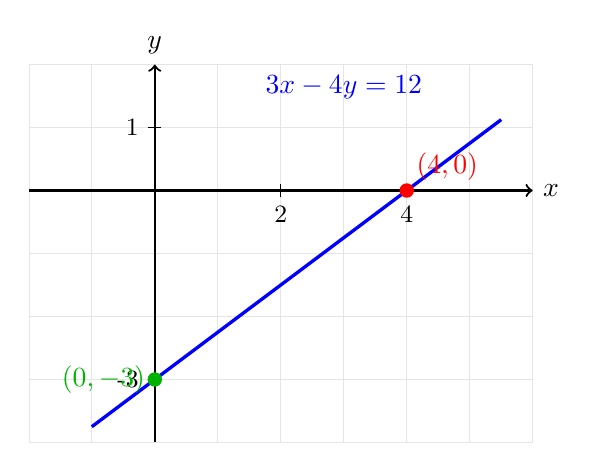
\begin{tikzpicture}[scale=0.8]
    % Grid
    \draw[gray!20, very thin] (-2,-4) grid (6,2);

    % Axes
    \draw[->, thick] (-2,0) -- (6,0) node[right] {$x$};
    \draw[->, thick] (0,-4) -- (0,2) node[above] {$y$};

    % Axis labels
    \foreach \x in {2,4}
        \draw (\x,0.1) -- (\x,-0.1) node[below, font=\small] {\x};
    \foreach \y in {-3,1}
        \draw (0.1,\y) -- (-0.1,\y) node[left, font=\small] {\y};

    % Plot the line 3x - 4y = 12
    \draw[blue, very thick, domain=-1:5.5] plot (\x, {(3*\x - 12)/4});

    % x-intercept
    \filldraw[red] (4,0) circle (3pt);
    \node[red, above right] at (4,0) {$(4,0)$};

    % y-intercept
    \filldraw[green!70!black] (0,-3) circle (3pt);
    \node[green!70!black, left] at (0,-3) {$(0,-3)$};

    % Equation label
    \node[blue, above] at (3,1.3) {$3x - 4y = 12$};
\end{tikzpicture}
\end{center}
\end{example}

\newpage

%========================================
% SECTION 11.4: Pendiente de una Recta
%========================================
\subsectiontitle{Pendiente de una Recta}

La pendiente es una medida de la inclinación de una recta.

\begin{definition}
\textbf{Pendiente de una Recta:}

La pendiente de una recta es una medida de su \textbf{inclinación}.

Para una recta no vertical que pasa por los puntos $(x_1, y_1)$ y $(x_2, y_2)$, la pendiente $m$ está dada por:

$$\boxed{m = \frac{\text{cambio vertical}}{\text{cambio horizontal}} = \frac{y_2 - y_1}{x_2 - x_1}}$$

donde $x_1 \neq x_2$ (la recta no es vertical).

\textbf{Interpretación geométrica:} La pendiente representa la razón entre el \textbf{cambio vertical} (rise) y el \textbf{cambio horizontal} (run) al movernos de un punto a otro sobre la recta.
\end{definition}

% Visual representation of slope
\begin{center}
\begin{tikzpicture}[scale=1.1]
    % Grid
    \draw[gray!20, very thin] (0,0) grid (8,6);

    % Axes
    \draw[->, thick] (0,0) -- (8,0) node[right] {$x$};
    \draw[->, thick] (0,0) -- (0,6) node[above] {$y$};

    % Points
    \def\xa{1}
    \def\ya{1}
    \def\xb{6}
    \def\yb{4}

    % Line through points
    \draw[blue, very thick] (0.5,0.7) -- (7,4.6);

    % Points
    \filldraw[red] (\xa,\ya) circle (3pt);
    \node[red, below left] at (\xa,\ya) {$(x_1, y_1)$};

    \filldraw[red] (\xb,\yb) circle (3pt);
    \node[red, above right] at (\xb,\yb) {$(x_2, y_2)$};

    % Right triangle showing rise and run
    \draw[dashed, green!70!black, thick] (\xa,\ya) -- (\xb,\ya);
    \draw[dashed, orange, thick] (\xb,\ya) -- (\xb,\yb);

    % Right angle mark
    \draw (\xb-0.3,\ya) -- (\xb-0.3,\ya+0.3) -- (\xb,\ya+0.3);

    % Labels for rise and run
    \draw[<->, green!70!black, thick] (\xa,\ya-0.5) -- (\xb,\ya-0.5);
    \node[green!70!black, below] at ({(\xa+\xb)/2},\ya-0.5) {\textbf{Cambio horizontal} = $x_2 - x_1$};

    \draw[<->, orange, thick] (\xb+0.5,\ya) -- (\xb+0.5,\yb);
    \node[orange, right] at (\xb+0.5,{(\ya+\yb)/2}) {\textbf{Cambio vertical} = $y_2 - y_1$};

    % Slope formula
    \node[purple, fill=white, draw, rounded corners] at (4,5.5) {$m = \dfrac{y_2 - y_1}{x_2 - x_1}$};
\end{tikzpicture}
\end{center}

\begin{example}
\textbf{Calcular la pendiente de una recta}

Calcule la pendiente de la recta que pasa por los puntos $(2, 1)$ y $(6, 5)$.

\textbf{Solución:}

Usamos $(x_1, y_1) = (2, 1)$ y $(x_2, y_2) = (6, 5)$.

\begin{align*}
m &= \frac{y_2 - y_1}{x_2 - x_1} \\
  &= \frac{5 - 1}{6 - 2} \\
  &= \frac{4}{4} \\
  &= 1
\end{align*}

\textbf{Respuesta:} La pendiente es $m = 1$.

\textbf{Nota:} El orden de los puntos no afecta el resultado. Si usamos $(x_1, y_1) = (6, 5)$ y $(x_2, y_2) = (2, 1)$:
$$m = \frac{1 - 5}{2 - 6} = \frac{-4}{-4} = 1$$
\end{example}

\newpage

\subsubsection*{Tipos de Pendientes}

Las rectas pueden tener diferentes tipos de pendientes según su inclinación:

% Visual comparison of different slope types
\begin{center}
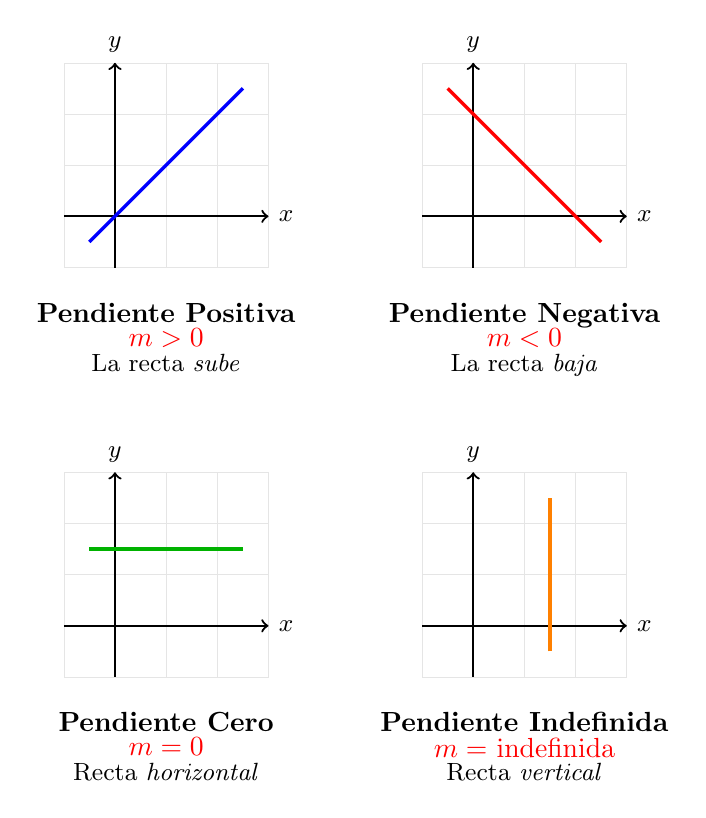
\begin{tikzpicture}[scale=0.65]
    % Positive slope (top left)
    \begin{scope}[xshift=0cm, yshift=0cm]
        \draw[gray!20, very thin] (-1,-1) grid (3,3);
        \draw[->, thick] (-1,0) -- (3,0) node[right, font=\small] {$x$};
        \draw[->, thick] (0,-1) -- (0,3) node[above, font=\small] {$y$};
        \draw[blue, very thick] (-0.5,-0.5) -- (2.5,2.5);
        \node[below] at (1,-1.5) {\textbf{Pendiente Positiva}};
        \node[below, red] at (1,-2) {$m > 0$};
        \node[below, font=\small] at (1,-2.5) {La recta \textit{sube}};
    \end{scope}

    % Negative slope (top right)
    \begin{scope}[xshift=7cm, yshift=0cm]
        \draw[gray!20, very thin] (-1,-1) grid (3,3);
        \draw[->, thick] (-1,0) -- (3,0) node[right, font=\small] {$x$};
        \draw[->, thick] (0,-1) -- (0,3) node[above, font=\small] {$y$};
        \draw[red, very thick] (-0.5,2.5) -- (2.5,-0.5);
        \node[below] at (1,-1.5) {\textbf{Pendiente Negativa}};
        \node[below, red] at (1,-2) {$m < 0$};
        \node[below, font=\small] at (1,-2.5) {La recta \textit{baja}};
    \end{scope}

    % Zero slope (bottom left)
    \begin{scope}[xshift=0cm, yshift=-8cm]
        \draw[gray!20, very thin] (-1,-1) grid (3,3);
        \draw[->, thick] (-1,0) -- (3,0) node[right, font=\small] {$x$};
        \draw[->, thick] (0,-1) -- (0,3) node[above, font=\small] {$y$};
        \draw[green!70!black, very thick] (-0.5,1.5) -- (2.5,1.5);
        \node[below] at (1,-1.5) {\textbf{Pendiente Cero}};
        \node[below, red] at (1,-2) {$m = 0$};
        \node[below, font=\small] at (1,-2.5) {Recta \textit{horizontal}};
    \end{scope}

    % Undefined slope (bottom right)
    \begin{scope}[xshift=7cm, yshift=-8cm]
        \draw[gray!20, very thin] (-1,-1) grid (3,3);
        \draw[->, thick] (-1,0) -- (3,0) node[right, font=\small] {$x$};
        \draw[->, thick] (0,-1) -- (0,3) node[above, font=\small] {$y$};
        \draw[orange, very thick] (1.5,-0.5) -- (1.5,2.5);
        \node[below] at (1,-1.5) {\textbf{Pendiente Indefinida}};
        \node[below, red] at (1,-2) {$m = $ indefinida};
        \node[below, font=\small] at (1,-2.5) {Recta \textit{vertical}};
    \end{scope}
\end{tikzpicture}
\end{center}

\begin{theorem}
\textbf{Casos Especiales de Pendiente:}

\begin{enumerate}
    \item \textbf{Recta Horizontal:} Todos los puntos tienen la misma coordenada $y$.
    \begin{itemize}
        \item Cambio vertical = 0
        \item $m = \dfrac{0}{\text{cambio horizontal}} = 0$
        \item Ecuación: $y = b$ (donde $b$ es constante)
    \end{itemize}

    \item \textbf{Recta Vertical:} Todos los puntos tienen la misma coordenada $x$.
    \begin{itemize}
        \item Cambio horizontal = 0
        \item $m = \dfrac{\text{cambio vertical}}{0} = $ indefinida
        \item Ecuación: $x = a$ (donde $a$ es constante)
    \end{itemize}
\end{enumerate}
\end{theorem}

\newpage

\begin{example}
\textbf{Identificar el tipo de pendiente}

Calcule la pendiente de la recta que pasa por cada par de puntos:

\textbf{a)} $(3, 2)$ y $(5, 8)$

\textbf{Solución:}
$$m = \frac{8 - 2}{5 - 3} = \frac{6}{2} = 3$$
Pendiente positiva ($m = 3$). La recta sube de izquierda a derecha.

\textbf{b)} $(-2, 5)$ y $(4, 5)$

\textbf{Solución:}
$$m = \frac{5 - 5}{4 - (-2)} = \frac{0}{6} = 0$$
Pendiente cero ($m = 0$). La recta es horizontal.

\textbf{c)} $(1, -3)$ y $(1, 7)$

\textbf{Solución:}
$$m = \frac{7 - (-3)}{1 - 1} = \frac{10}{0} = \text{indefinida}$$
Pendiente indefinida. La recta es vertical.

\textbf{d)} $(0, 4)$ y $(3, -2)$

\textbf{Solución:}
$$m = \frac{-2 - 4}{3 - 0} = \frac{-6}{3} = -2$$
Pendiente negativa ($m = -2$). La recta baja de izquierda a derecha.
\end{example}

\newpage

%========================================
% SECTION 11.5: Formas de la Ecuación de una Recta
%========================================
\subsectiontitle{Formas de la Ecuación de una Recta}

Existen varias formas de escribir la ecuación de una recta, cada una útil en diferentes situaciones.

\subsubsection*{Forma Pendiente-Intersecto}

\begin{definition}
\textbf{Forma Pendiente-Intersecto (Slope-Intercept Form):}

$$\boxed{y = mx + b}$$

donde:
\begin{itemize}
    \item $m$ es la \textbf{pendiente} de la recta
    \item $b$ es la \textbf{intersección con el eje $y$} (y-intercept)
    \item La recta pasa por el punto $(0, b)$
\end{itemize}

Esta es la forma más útil porque nos permite identificar inmediatamente la pendiente y la intersección con el eje $y$.
\end{definition}

% Visual representation of y = mx + b
\begin{center}
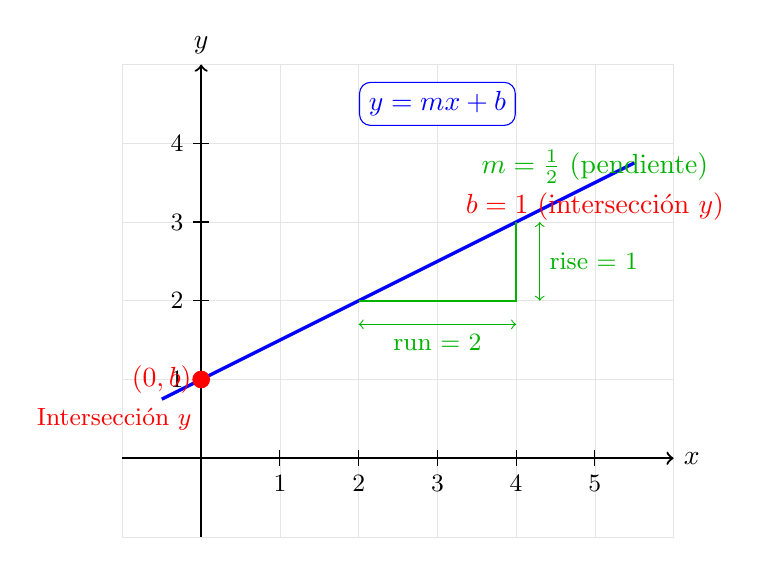
\begin{tikzpicture}[scale=1.0]
    % Grid
    \draw[gray!20, very thin] (-1,-1) grid (6,5);

    % Axes
    \draw[->, thick] (-1,0) -- (6,0) node[right] {$x$};
    \draw[->, thick] (0,-1) -- (0,5) node[above] {$y$};

    % Axis labels
    \foreach \x in {1,2,3,4,5}
        \draw (\x,0.1) -- (\x,-0.1) node[below, font=\small] {\x};
    \foreach \y in {1,2,3,4}
        \draw (0.1,\y) -- (-0.1,\y) node[left, font=\small] {\y};

    % Plot y = 0.5x + 1
    \draw[blue, very thick, domain=-0.5:5.5] plot (\x, {0.5*\x + 1});

    % y-intercept
    \filldraw[red] (0,1) circle (3pt);
    \node[red, left] at (0,1) {$(0, b)$};
    \node[red, left] at (0,0.5) {\small Intersección $y$};

    % Slope triangle
    \draw[green!70!black, thick] (2,2) -- (4,2) -- (4,3);
    \draw[<->, green!70!black] (2,1.7) -- (4,1.7);
    \node[green!70!black, below] at (3,1.7) {\small run = 2};
    \draw[<->, green!70!black] (4.3,2) -- (4.3,3);
    \node[green!70!black, right] at (4.3,2.5) {\small rise = 1};

    % Equation and components
    \node[blue, fill=white, draw, rounded corners] at (3,4.5) {$y = mx + b$};
    \node[green!70!black] at (5,3.7) {$m = \frac{1}{2}$ (pendiente)};
    \node[red] at (5,3.2) {$b = 1$ (intersección $y$)};
\end{tikzpicture}
\end{center}

\begin{example}
\textbf{Graficar usando la forma pendiente-intersecto}

Grafique la ecuación $y = 2x - 3$.

\textbf{Solución:}

Identificamos:
\begin{itemize}
    \item Pendiente: $m = 2 = \dfrac{2}{1}$ (sube 2 unidades por cada 1 unidad a la derecha)
    \item Intersección con el eje $y$: $b = -3$
\end{itemize}

\textbf{Pasos para graficar:}
\begin{enumerate}
    \item Graficar el punto $(0, -3)$ (la intersección con el eje $y$)
    \item Desde ese punto, usar la pendiente: subir 2 unidades y moverse 1 unidad a la derecha
    \item Esto nos da el punto $(1, -1)$
    \item Trazar la recta que pasa por ambos puntos
\end{enumerate}

\begin{center}
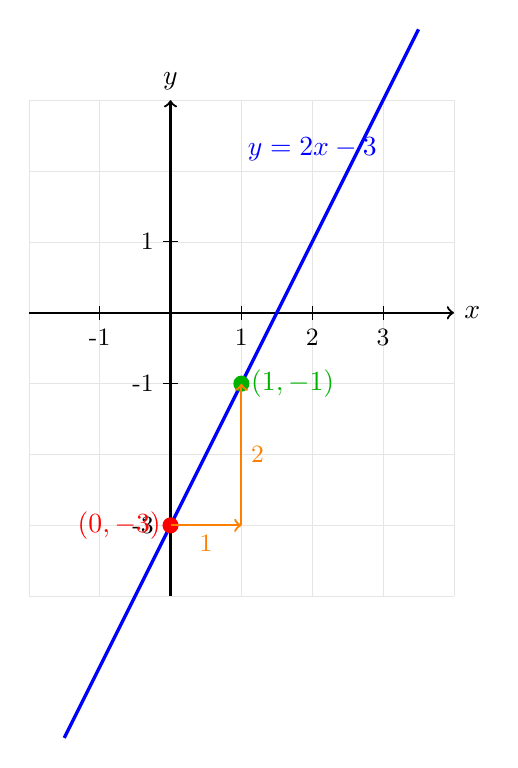
\begin{tikzpicture}[scale=0.9]
    % Grid
    \draw[gray!20, very thin] (-2,-4) grid (4,3);

    % Axes
    \draw[->, thick] (-2,0) -- (4,0) node[right] {$x$};
    \draw[->, thick] (0,-4) -- (0,3) node[above] {$y$};

    % Axis labels
    \foreach \x in {-1,1,2,3}
        \draw (\x,0.1) -- (\x,-0.1) node[below, font=\small] {\x};
    \foreach \y in {-3,-1,1}
        \draw (0.1,\y) -- (-0.1,\y) node[left, font=\small] {\y};

    % Plot the line
    \draw[blue, very thick, domain=-1.5:3.5] plot (\x, {2*\x - 3});

    % y-intercept
    \filldraw[red] (0,-3) circle (3pt);
    \node[red, left] at (0,-3) {$(0,-3)$};

    % Second point
    \filldraw[green!70!black] (1,-1) circle (3pt);
    \node[green!70!black, right] at (1,-1) {$(1,-1)$};

    % Slope visualization
    \draw[orange, thick, ->] (0,-3) -- (1,-3);
    \node[orange, below] at (0.5,-3) {\small 1};
    \draw[orange, thick, ->] (1,-3) -- (1,-1);
    \node[orange, right] at (1,-2) {\small 2};

    % Equation
    \node[blue, above] at (2,2) {$y = 2x - 3$};
\end{tikzpicture}
\end{center}
\end{example}

\newpage

\subsubsection*{Forma Punto-Pendiente}

\begin{definition}
\textbf{Forma Punto-Pendiente (Point-Slope Form):}

Si conocemos la pendiente $m$ de una recta y un punto $(x_1, y_1)$ por donde pasa, la ecuación es:

$$\boxed{y - y_1 = m(x - x_1)}$$

donde:
\begin{itemize}
    \item $m$ es la pendiente
    \item $(x_1, y_1)$ es un punto conocido de la recta
\end{itemize}

Esta forma es útil cuando conocemos un punto y la pendiente, pero no la intersección con el eje $y$.
\end{definition}

\begin{example}
\textbf{Escribir la ecuación usando forma punto-pendiente}

Encuentre la ecuación de la recta que tiene pendiente $m = 3$ y pasa por el punto $(2, 5)$.

\textbf{Solución:}

Usamos la forma punto-pendiente con $m = 3$, $x_1 = 2$, $y_1 = 5$:

\begin{align*}
y - y_1 &= m(x - x_1) \\
y - 5 &= 3(x - 2)
\end{align*}

Esta es la ecuación en forma punto-pendiente.

\textbf{Convertir a forma pendiente-intersecto:}
\begin{align*}
y - 5 &= 3(x - 2) \\
y - 5 &= 3x - 6 \\
y &= 3x - 6 + 5 \\
y &= 3x - 1
\end{align*}

\textbf{Respuesta:} $y - 5 = 3(x - 2)$ o $y = 3x - 1$
\end{example}

\begin{example}
\textbf{Encontrar la ecuación dados dos puntos}

Encuentre la ecuación de la recta que pasa por los puntos $(-1, 4)$ y $(3, -2)$.

\textbf{Solución:}

\textbf{Paso 1:} Calcular la pendiente
$$m = \frac{-2 - 4}{3 - (-1)} = \frac{-6}{4} = -\frac{3}{2}$$

\textbf{Paso 2:} Usar la forma punto-pendiente con uno de los puntos (usaremos $(-1, 4)$)
\begin{align*}
y - y_1 &= m(x - x_1) \\
y - 4 &= -\frac{3}{2}(x - (-1)) \\
y - 4 &= -\frac{3}{2}(x + 1)
\end{align*}

\textbf{Paso 3:} Convertir a forma pendiente-intersecto
\begin{align*}
y - 4 &= -\frac{3}{2}x - \frac{3}{2} \\
y &= -\frac{3}{2}x - \frac{3}{2} + 4 \\
y &= -\frac{3}{2}x + \frac{5}{2}
\end{align*}

\textbf{Respuesta:} $y = -\dfrac{3}{2}x + \dfrac{5}{2}$
\end{example}

\newpage

\subsubsection*{Resumen de Formas de Ecuaciones de Rectas}

\begin{center}
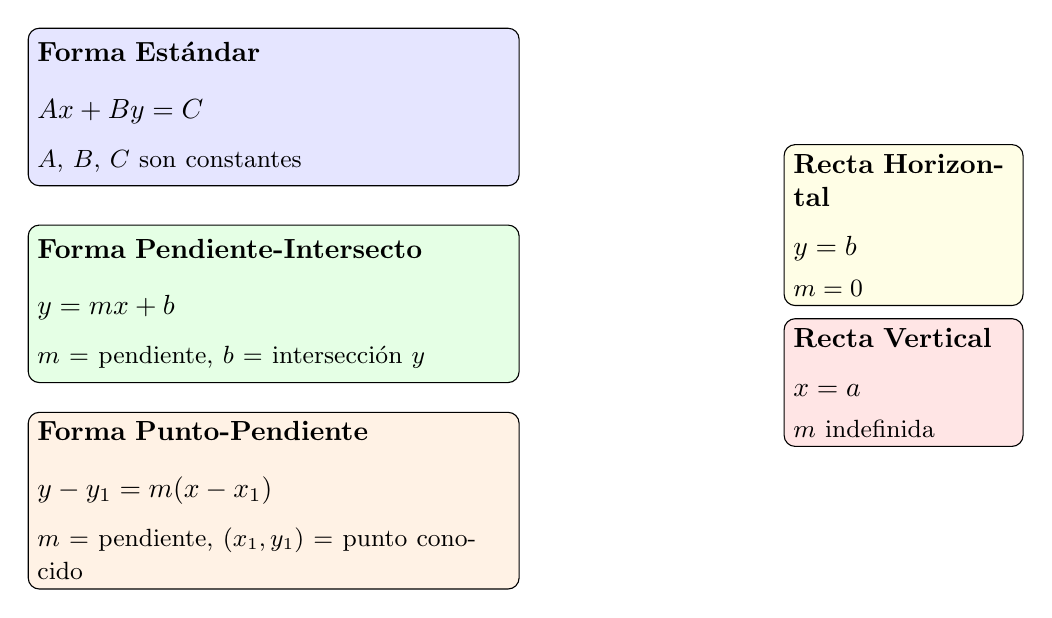
\begin{tikzpicture}
    % Standard form
    \node[draw, fill=blue!10, text width=6cm, minimum height=2cm, rounded corners] at (0,4) {
        \textbf{Forma Estándar} \\[0.3cm]
        $Ax + By = C$ \\[0.2cm]
        \small $A$, $B$, $C$ son constantes
    };

    % Slope-intercept form
    \node[draw, fill=green!10, text width=6cm, minimum height=2cm, rounded corners] at (0,1.5) {
        \textbf{Forma Pendiente-Intersecto} \\[0.3cm]
        $y = mx + b$ \\[0.2cm]
        \small $m$ = pendiente, $b$ = intersección $y$
    };

    % Point-slope form
    \node[draw, fill=orange!10, text width=6cm, minimum height=2cm, rounded corners] at (0,-1) {
        \textbf{Forma Punto-Pendiente} \\[0.3cm]
        $y - y_1 = m(x - x_1)$ \\[0.2cm]
        \small $m$ = pendiente, $(x_1, y_1)$ = punto conocido
    };

    % Horizontal line
    \node[draw, fill=yellow!10, text width=2.8cm, minimum height=1.5cm, rounded corners] at (8,2.5) {
        \textbf{Recta Horizontal} \\[0.2cm]
        $y = b$ \\[0.1cm]
        \small $m = 0$
    };

    % Vertical line
    \node[draw, fill=red!10, text width=2.8cm, minimum height=1.5cm, rounded corners] at (8,0.5) {
        \textbf{Recta Vertical} \\[0.2cm]
        $x = a$ \\[0.1cm]
        \small $m$ indefinida
    };
\end{tikzpicture}
\end{center}

\begin{theorem}
\textbf{Rectas Paralelas y Perpendiculares:}

\begin{enumerate}
    \item \textbf{Rectas Paralelas:} Dos rectas no verticales son paralelas si y solo si tienen la \textbf{misma pendiente}.
    $$\text{Si } L_1 \parallel L_2, \text{ entonces } m_1 = m_2$$

    \item \textbf{Rectas Perpendiculares:} Dos rectas no verticales son perpendiculares si y solo si sus pendientes son \textbf{recíprocas negativas}.
    $$\text{Si } L_1 \perp L_2, \text{ entonces } m_1 \cdot m_2 = -1 \text{ o } m_2 = -\frac{1}{m_1}$$
\end{enumerate}
\end{theorem}

% Visual representation of parallel and perpendicular lines
\begin{center}
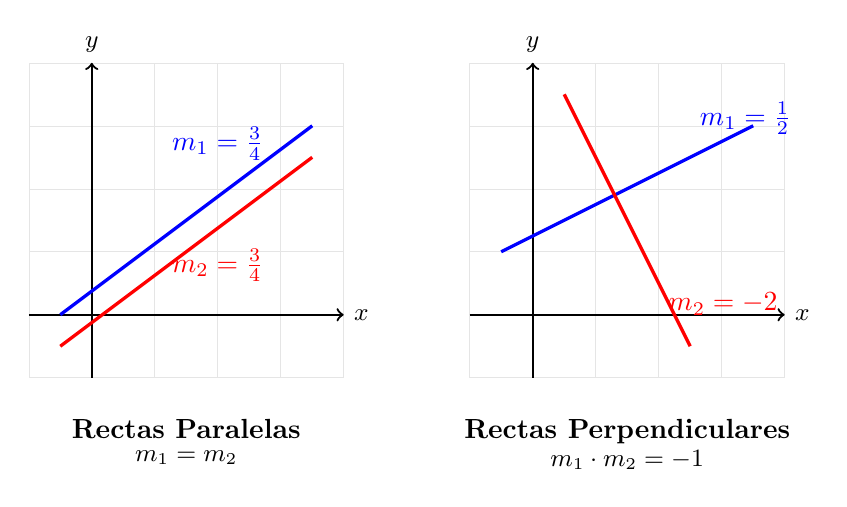
\begin{tikzpicture}[scale=0.8]
    % Parallel lines
    \begin{scope}[xshift=0cm]
        \draw[gray!20, very thin] (-1,-1) grid (4,4);
        \draw[->, thick] (-1,0) -- (4,0) node[right, font=\small] {$x$};
        \draw[->, thick] (0,-1) -- (0,4) node[above, font=\small] {$y$};

        \draw[blue, very thick] (-0.5,0) -- (3.5,3);
        \node[blue, above] at (2,2.3) {$m_1 = \frac{3}{4}$};

        \draw[red, very thick] (-0.5,-0.5) -- (3.5,2.5);
        \node[red, below] at (2,1.2) {$m_2 = \frac{3}{4}$};

        \node[below] at (1.5,-1.5) {\textbf{Rectas Paralelas}};
        \node[below, font=\small] at (1.5,-2) {$m_1 = m_2$};
    \end{scope}

    % Perpendicular lines
    \begin{scope}[xshift=7cm]
        \draw[gray!20, very thin] (-1,-1) grid (4,4);
        \draw[->, thick] (-1,0) -- (4,0) node[right, font=\small] {$x$};
        \draw[->, thick] (0,-1) -- (0,4) node[above, font=\small] {$y$};

        \draw[blue, very thick] (-0.5,1) -- (3.5,3);
        \node[blue, above right] at (2.5,2.7) {$m_1 = \frac{1}{2}$};

        \draw[red, very thick] (0.5,3.5) -- (2.5,-0.5);
        \node[red, below right] at (2,0.5) {$m_2 = -2$};

        \node[below] at (1.5,-1.5) {\textbf{Rectas Perpendiculares}};
        \node[below, font=\small] at (1.5,-2) {$m_1 \cdot m_2 = -1$};
    \end{scope}
\end{tikzpicture}
\end{center}

\begin{example}
\textbf{Identificar rectas paralelas y perpendiculares}

Considere las rectas $L_1: y = 2x + 3$, $L_2: y = 2x - 5$, y $L_3: y = -\dfrac{1}{2}x + 1$.

\textbf{a)} ¿Son $L_1$ y $L_2$ paralelas?

\textbf{Solución:} Ambas tienen pendiente $m = 2$. Como $m_1 = m_2 = 2$, las rectas \textbf{SÍ son paralelas}.

\textbf{b)} ¿Son $L_1$ y $L_3$ perpendiculares?

\textbf{Solución:} $m_1 = 2$ y $m_3 = -\dfrac{1}{2}$. Verificamos:
$$m_1 \cdot m_3 = 2 \cdot \left(-\frac{1}{2}\right) = -1$$

Como el producto es $-1$, las rectas \textbf{SÍ son perpendiculares}.
\end{example}

\textbf{Notas Importantes:}
\begin{itemize}
    \item Una recta horizontal ($y = b$) y una recta vertical ($x = a$) son siempre perpendiculares
    \item Dos rectas verticales son paralelas
    \item Dos rectas horizontales son paralelas
    \item La forma pendiente-intersecto es la más útil para identificar rápidamente la pendiente
    \item Convertir entre formas es una habilidad importante en álgebra
\end{itemize}
